\section{Introduction}
\label{sec:intro}

Foundation models represent a significant advancement in the field of artificial intelligence and machine learning due to their ability to serve as a versatile base for a wide range of tasks and applications. The models are pretrained on large, diverse datasets in a self supervised manner, allowing them to learn general features and patterns. This pretraining stage enables the models to perform well on various downstream tasks with minimal additional fine-tuning, reducing the need for extensive labeled datasets for each specific task. \cite{foundationModels} \\
In the context of Earth observation, unlabeled data is often abundant, while labeled data is scarce, particularly in geolocated datasets such as those used in remote sensing \cite{geoAwareSelfSuper}. Foundation models are highly valuable in this field because they can be pretrained without the need for labels, using un-supervised or self-supervised learning techniques. \\
When evaluating a foundation model, the quality of the learned features is important. There are two main types of evaluation: intrinsic and extrinsic. Intrinsic evaluation assesses the model based solely on the learned features, focusing on their expressiveness and quality. In contrast, extrinsic evaluation measures the model's performance on an external downstream task. \cite{foundationModels} \\
This paper analyses the application of selected foundation models on the BigEarthNet dataset \cite{bigEartNetMM} using both types of evaluation. The external downstream task is multi-label classification. Fig. \ref{fig:setup} illustrates the evaluation setup.

\begin{figure}[t]
  \centering
   %\fbox{\rule{0pt}{1.5in} \rule{0.9\linewidth}{0pt}}
   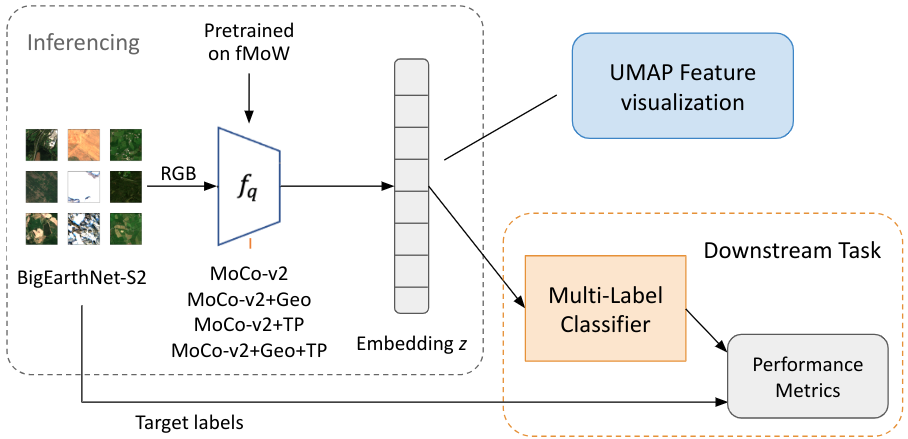
\includegraphics[width=\linewidth]{figures/ExperimentSetup.png}
   \caption{Illustration of the evaluation experiments on the BigEarthNet dataset: The query encoder of the examined MoCo-v2 based foundation models is used to extract featuress $z$, which are then evaluated through UMAP feature visualization and the performance of a classifier on the multi-label classification downstream task.}
   \label{fig:setup}
\end{figure}

